%%%%%%%% ICML 2025 EXAMPLE LATEX SUBMISSION FILE %%%%%%%%%%%%%%%%%

\documentclass{article}

% Recommended, but optional, packages for figures and better typesetting:
\usepackage{microtype}
\usepackage{graphicx}
\usepackage{subfigure}
\usepackage{stfloats}

\usepackage{booktabs} % for professional tables

\usepackage{hyperref}


\newcommand{\theHalgorithm}{\arabic{algorithm}}

% Use the following line for the initial blind version submitted for review:
% \usepackage{icml2025}

% If accepted, instead use the following line for the camera-ready submission:
\usepackage[accepted]{icml2025}

% For theorems and such
\usepackage{amsmath}
\usepackage{amssymb}
\usepackage{mathtools}
\usepackage{amsthm}

% if you use cleveref..
\usepackage[capitalize,noabbrev]{cleveref}

%%%%%%%%%%%%%%%%%%%%%%%%%%%%%%%%
% THEOREMS
%%%%%%%%%%%%%%%%%%%%%%%%%%%%%%%%
\theoremstyle{plain}
\newtheorem{theorem}{Theorem}[section]
\newtheorem{proposition}[theorem]{Proposition}
\newtheorem{lemma}[theorem]{Lemma}
\newtheorem{corollary}[theorem]{Corollary}
\theoremstyle{definition}
\newtheorem{definition}[theorem]{Definition}
\newtheorem{assumption}[theorem]{Assumption}
\theoremstyle{remark}
\newtheorem{remark}[theorem]{Remark}

% Todonotes is useful during development; simply uncomment the next line
%    and comment out the line below the next line to turn off comments
%\usepackage[disable,textsize=tiny]{todonotes}
\usepackage[textsize=tiny]{todonotes}


% The \icmltitle you define below is probably too long as a header.
% Therefore, a short form for the running title is supplied here:
\icmltitlerunning{Measurement of Cellular Call Performance}

\begin{document}

\twocolumn[
\icmltitle{Measurement of Cellular Call Performance}


\icmlsetsymbol{equal}{*}

\begin{icmlauthorlist}
\icmlauthor{Gaurav Kumar}{equal,yyy}
\icmlauthor{Shiv Narang}{equal,yyy}
\end{icmlauthorlist}


\icmlaffiliation{yyy}{Department of CSE, IIT Bombay, Mumbai, India}

\icmlcorrespondingauthor{Gaurav Kumar}{23b0989@iitb.ac.in}
\icmlcorrespondingauthor{Shiv Narang}{23b0989@iitb.ac.in}

% You may provide any keywords that you
% find helpful for describing your paper; these are used to populate
% the "keywords" metadata in the PDF but will not be shown in the document
\icmlkeywords{Machine Learning, ICML}

\vskip 0.3in
]




\begin{abstract}
We present a mobile system for collecting and analyzing user-reported feedback on cellular call quality. The system integrates an Android-based client that captures post-call subjective feedback alongside automatically collected network metadata, including signal strength, network type, and location. This combined dataset enables large-scale analysis of call performance across carriers and environments. By correlating user experience with objective network conditions, our framework provides a foundation for identifying patterns in call quality and supports data-driven evaluation of cellular network performance. The source code is available at \url{https://github.com/gkonethree/CallFeedbackApp}
\end{abstract}


\section{Introduction}

Cellular call quality remains a critical component of user experience, yet it is difficult to measure reliably at scale due to the lack of fine-grained, user-level feedback combined with network-level context. 

In this work, we develop a mobile application that systematically collects post-call feedback from users while simultaneously recording relevant network and device metadata. The system captures both subjective inputs, such as perceived voice quality and reported issues, and objective measurements, including signal strength, network generation, and approximate location. This dual perspective enables a more comprehensive understanding of call performance in real-world conditions.

The collected data is transmitted to a backend service for storage and further analysis. By aggregating feedback across users, locations, and network conditions, the system enables large-scale evaluation of cellular performance and user satisfaction. This dataset serves as the basis for analysis, including identifying correlations between network characteristics and perceived call quality, as well as uncovering patterns across carriers and environments.


\section{Tech Stack}

The system is implemented using a lightweight and modular technology stack.

The mobile client is developed in Kotlin, the primary programming language for Android application development. Kotlin provides strong interoperability with existing Android APIs and enables concise and maintainable code. Development is carried out using Android Studio.

The backend service is implemented using FastAPI, a high-performance Python framework for building RESTful APIs. FastAPI is chosen for its simplicity, asynchronous capabilities, and strong support for data validation through Pydantic schemas. 

MongoDB is used as the primary database for storing feedback records.

For deployment, the backend is containerized using Docker, ensuring portability and ease of deployment across different environments.

\section{App Workflow}

The mobile application operates as a foreground service that reacts to telephony state changes in an event-driven manner. Instead of continuously polling the device state, the system relies on Android’s telephony framework to notify the application of call state transitions via registered listeners or broadcast receivers.

When a call transitions from an active state (\texttt{CALL\_STATE\_OFFHOOK}) to an idle state (\texttt{CALL\_STATE\_IDLE}), the application infers that the call has ended. This transition event triggers the feedback workflow, upon which an overlay interface is displayed to prompt the user for input.

Simultaneously, the application retrieves relevant device and network metadata, including signal strength, network type, and location (subject to user permissions). This data collection is performed at the time of the event and does not require continuous monitoring.

Once the user submits the feedback, the collected data is transmitted to the backend via an HTTP POST request. The backend validates the request and stores the data for subsequent analysis.

Authentication is implemented using an API key mechanism. Each client request includes an API key in the request headers, which is validated by the backend before processing. This approach provides a simple and effective method for controlling access to the API.

\section{User Interface Design}
The mobile application provides an overlay-based feedback interface that appears after a call ends. The UI is designed to be minimal and easily dismissible.

\begin{figure}[h!]
    \centering
    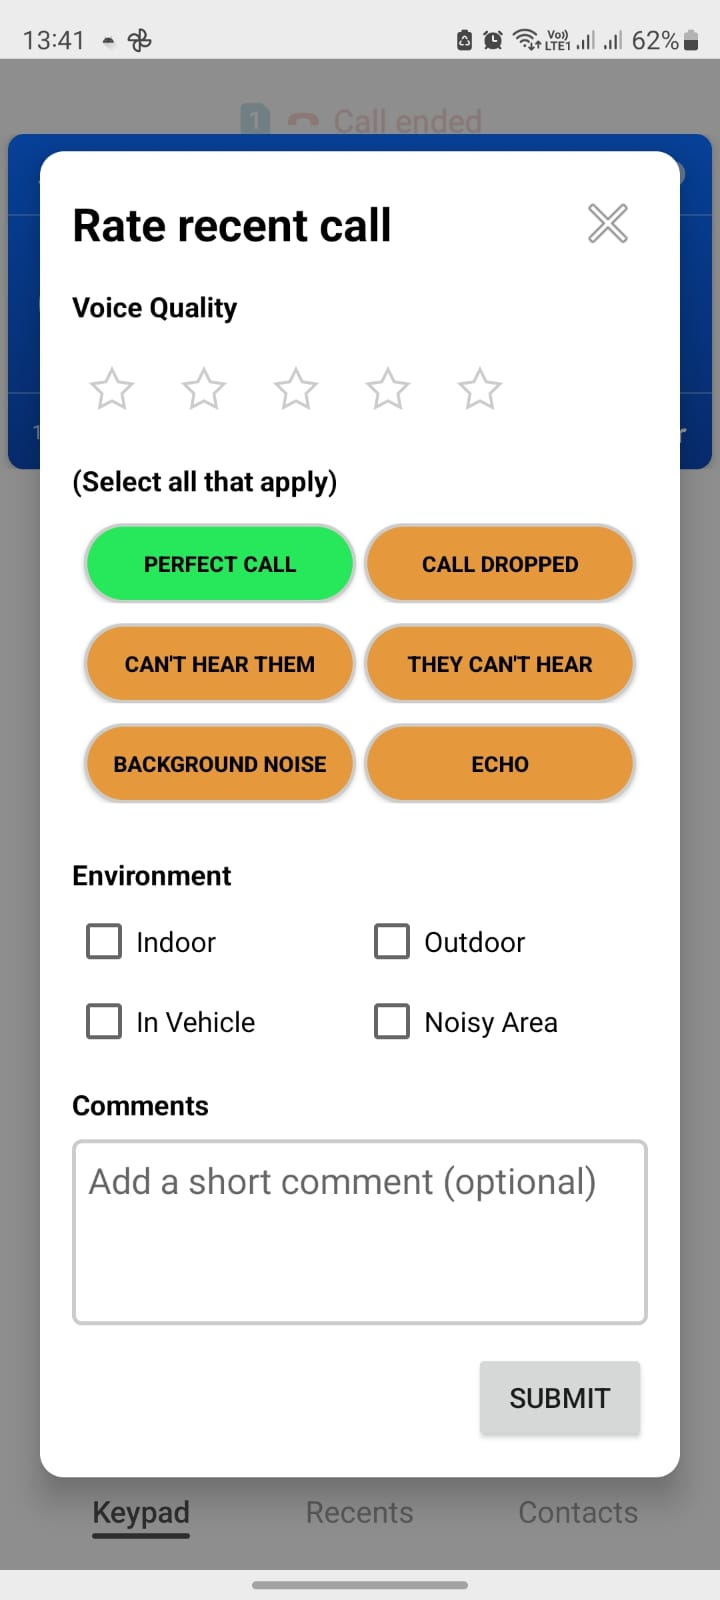
\includegraphics[width=0.25\textwidth]{unmarked.jpeg}
    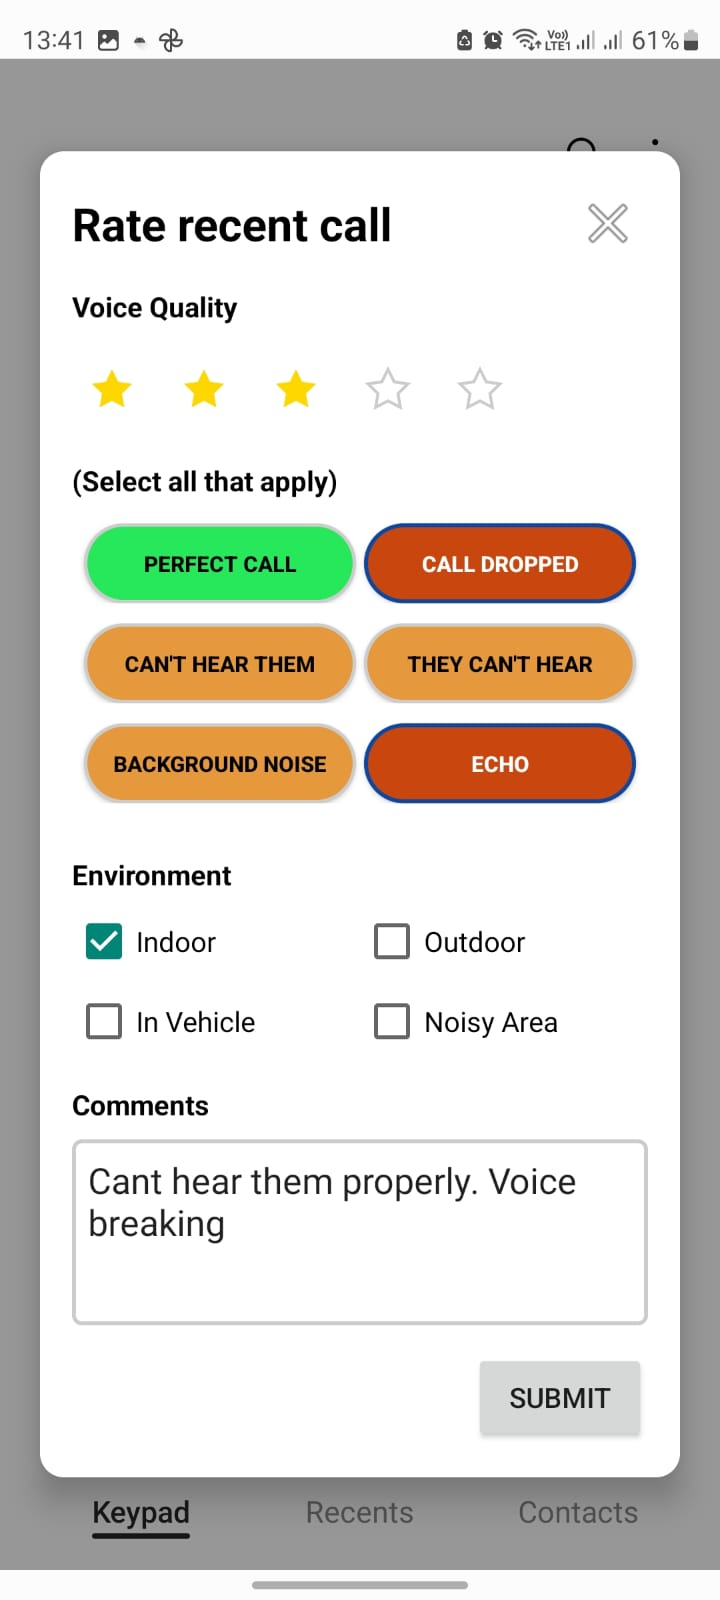
\includegraphics[width=0.25\textwidth]{marked.jpeg}
    \caption{User interface flow: overlay feedback screen}
    \label{fig:ui_flow}
\end{figure}

\subsection{User Interface Flow}
The Android application registers a call state listener with the \texttt{TelephonyManager} API, allowing the Android telephony framework to asynchronously notify the application whenever a call state change occurs. When a transition from \\ \texttt{CALL\_STATE\_OFFHOOK} to \texttt{CALL\_STATE\_IDLE} is detected, the system infers that a call has ended and triggers the feedback flow.

This event-driven approach ensures that the feedback UI is displayed only after the call is completed, avoiding user interruption during the call.

\subsection{Feedback Screen Layout}

The feedback interface is designed to be simple, fast, and easily accessible. The layout consists of:

\begin{itemize}
    \item A prominent heading indicating that feedback is requested.
    \item Star-based rating components for quantitative feedback such as voice quality.
    \item Optional categorical selections for audio issues and call environment.
    \item A submit button to send feedback to the backend.
\end{itemize}

Star ratings are intentionally sized larger than default UI components to improve touch accuracy and encourage user participation.

\subsection{User Interaction Flow}

The interaction flow is as follows:
\begin{enumerate}
    \item Call ends and call state listener is triggered.
    \item Feedback activity or bottom sheet is launched.
    \item User provides ratings and optional inputs.
    \item Feedback data is submitted asynchronously.
    \item UI closes automatically upon successful submission.
\end{enumerate}

All input fields are optional to minimize friction and prevent feedback abandonment.

\subsection{Metadata Collection}

Alongside user input, the client automatically collects device and network metadata at the time of feedback submission, including:
\begin{itemize}
    \item Carrier Name
    \item Network type (WiFi, 2G, 3G, 4G, 5G).
    \item Signal strength in dBm.
    \item Approximate geographic location 
    \item Call Duration
    \item Timestamp of feedback submission.
\end{itemize}
This data is collected without additional user interaction.\\


\section{Feedback}

\subsection{User Feedback}
The overlay with user feedback has the following:
\begin{itemize}
    \item \textbf{Voice Quality} Rating stars from 1-5
    \item \textbf{Audio Issues} Multiple selectable options including Perfect Call, Call Dropped, Can't Hear them, They can't hear, background noise, echo.
    \item \textbf{Environment} Single selectable from Indoor, Outdoor, In Vehicle, Noisy Area.
    \item \textbf{Comments} Additional subjective feedback by the user
\end{itemize}
All these fields are optional with default null values.

\subsection{Device Reported Data}
We try to record the following from device:
\begin{itemize}
    \item \textbf{Network Generation} Check if user is on WiFi or Celluar, and if on cellular, report generation also.
    \item \textbf{Signal Strength} Check the signal strength in dBm. This measurement is sometimes blocked by the device due to security reasons.
    \item \textbf{Location} We also try to fetch the last known exact location (or approximate, if exact not available).
\end{itemize}

\section{APIs Used}

This section describes the Android platform APIs used to collect network, radio, and contextual metadata for post-call analysis.

\subsection{TelephonyManager}

The \texttt{TelephonyManager} API provides access to cellular network and radio-related information. It is used to determine the current cellular network type and signal strength.

\subsubsection{Call State Detection}

Call state detection is performed using the \texttt{TelephonyManager} API to monitor changes in the device's telephony call state. The Android system reports call state transitions via a listener mechanism, allowing applications to react to call lifecycle events in real time.

The primary call states are represented by integer constants defined in \texttt{TelephonyManager}:
\begin{itemize}
    \item \texttt{CALL\_STATE\_IDLE}: Indicates that the device is not currently involved in a call.
    \item \texttt{CALL\_STATE\_RINGING}: Indicates an incoming call is ringing.
    \item \texttt{CALL\_STATE\_OFFHOOK}: Indicates that a call is active, including outgoing calls or answered incoming calls.
\end{itemize}

Call state updates are received by registering a \texttt{PhoneStateListener}(or \texttt{CallStateListener} for newer versions) and overriding the \texttt{onCallStateChanged()} callback. Transitions between these states allow the application to infer call start and call end events. Specifically, a transition to \texttt{CALL\_STATE\_OFFHOOK} is interpreted as the start of a call, while a transition back to \texttt{CALL\_STATE\_IDLE} signifies the termination of a call.


% Although \texttt{PhoneStateListener} is marked as deprecated in newer Android versions, it remains the most reliable and widely supported approach for call state monitoring across a broad range of devices and API levels.


\subsubsection{Network Type Detection}

The API method \texttt{getDataNetworkType()} returns an integer constant representing the current radio access technology. These values are mapped to high-level network generations as follows:

\begin{itemize}
    \item \textbf{2G}: GPRS, EDGE, CDMA, 1xRTT, IDEN
    \item \textbf{3G}: UMTS, HSDPA, HSUPA, HSPA, EVDO variants
    \item \textbf{4G/LTE}: LTE
    \item \textbf{5G/NR}: NR
\end{itemize}


\subsubsection{Signal Strength Estimation}

The \texttt{allCellInfo} API is used to retrieve a list of available cell information objects. Depending on the radio technology, the signal strength is extracted from the corresponding classes:

\begin{itemize}
    \item \texttt{CellInfoGsm}
    \item \texttt{CellInfoWcdma}
    \item \texttt{CellInfoLte}
    \item \texttt{CellInfoNr} (Android 12+)
\end{itemize}

The received signal strength indicator , expressed in dBm, is extracted from the \texttt{CellSignalStrength} object. Invalid or unavailable values are filtered before use.

\subsection{ConnectivityManager}

The \texttt{ConnectivityManager} API is used to determine the currently active network transport.

Using \texttt{getActiveNetwork()} and \texttt{getNetworkCapabilities()}, the application identifies whether the device is connected via:

\begin{itemize}
    \item \textbf{Wi-Fi} (\texttt{TRANSPORT\_WIFI})
    \item \textbf{Cellular} (\texttt{TRANSPORT\_CELLULAR})
\end{itemize}


\subsection{FusedLocationProviderClient}

The \texttt{FusedLocationProviderClient} API from Google Play Services is used to obtain the device’s approximate geographical location at the time of feedback submission.

The method \texttt{getCurrentLocation()} is invoked with \texttt{PRIORITY\_BALANCED\_POWER\_ACCURACY}, which provides a coarse location estimate while minimizing battery consumption. Location access is performed only when the appropriate runtime permissions are granted.


\section{App as a foreground service}

\subsection{Background Execution Constraints in Android}

Modern Android versions (Android 8.0 and above) impose strict limitations on background execution in order to improve battery life and system stability. Applications running in the background may be:

\begin{itemize}
    \item Stopped due to memory pressure,
    \item Restricted from receiving broadcasts,
    \item Prevented from executing long-running background tasks.
\end{itemize}

In the context of this application, background execution restrictions can interrupt call detection and feedback collection. Therefore, we design the app to be a foreground service with persistent notification.

\subsection{Persistent Notification Requirement}

Android enforces that every foreground service must display a non-dismissible notification.

In this application, the notification indicates:

\begin{itemize}
    \item ``Call monitor active'' when idle,
    \item ``Monitoring call quality'' during an active call.
\end{itemize}

Instead of stopping the foreground service after each call, the notification is updated dynamically. 

\subsection{System Stability Considerations}

If a service is started using \texttt{startForegroundService()}, Android requires that \texttt{startForeground()} be invoked within five seconds. Failure to do so results in a \texttt{ForegroundServiceDidNotStartInTimeException}, causing application crashes and system-level instability warnings.

To comply with this requirement, the application:

\begin{itemize}
    \item Immediately starts in foreground mode upon creation,
    \item Maintains a minimal persistent notification,
    \item Updates the notification during call state transitions,
    \item Avoids unnecessary stopping and restarting of the service.
\end{itemize}

Although it introduces a persistent notification, this approach guarantees correctness, reliability.


\section{Backend Design}

The backend is implemented as a RESTful web service using \texttt{FastAPI}. 
The backend exposes endpoints for:
\begin{itemize}
    \item Submitting new feedback records.
    \item Retrieving stored feedback with pagination support.
\end{itemize}
All incoming requests are validated against predefined schemas to ensure data consistency and prevent malformed inputs.

Feedback data is represented using structured schemas that combine:
\begin{itemize}
    \item Subjective user feedback (ratings, issues, environment).
    \item Objective device metadata (network type, signal strength, location).
\end{itemize}

\section{Data Collection}

The application was initially evaluated through an internal testing phase lasting approximately one to two weeks. During this phase, the system was used extensively to identify and resolve minor functional and usability issues, resulting in a stable release build.

Following internal validation, the application was deployed in a pilot study involving a small group of five participants. Participants used devices on multiple cellular carriers, including Airtel, Vodafone Idea (VI), and Jio, allowing preliminary coverage of different network providers.

Prior to participation, all users provided informed consent for data collection. The application was installed on participant devices via a distributed APK file.

Data collection was conducted over a period of two weeks, during which approximately 90 feedback instances were recorded. 

Although limited in scale, this pilot dataset provides an initial basis for analyzing relationships between perceived call quality and underlying network conditions.

\subsection{Security and Privacy Considerations}

The system is designed with consideration of user privacy:

\begin{itemize}
    \item No call content, audio recordings, or phone numbers are collected or stored.
    \item Location data is collected only when explicitly permitted by the user through runtime permissions.
    \item All feedback inputs are voluntary, and users may choose to skip any or all fields.
\end{itemize}

The application operates without interfering with normal device usage, and feedback collection is performed only after call completion to avoid disrupting ongoing communication.
\section{Results}

We first analyze the average voice quality ratings reported by users across different carriers, as shown in \autoref{fig:vc}. Overall, all carriers achieve an average rating above 4, indicating generally satisfactory call quality during the pilot study. Among the three carriers, Airtel achieves the highest average voice quality rating, suggesting comparatively better user-perceived call experience.

\begin{figure}[t]
    \centering
    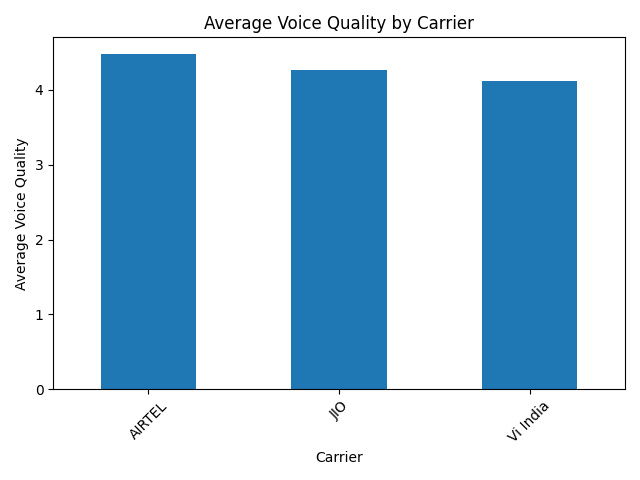
\includegraphics[width=0.5\linewidth]{avg_voice_quality_by_carrier.png}
    \caption{Average voice quality rating across carriers}
    \label{fig:vc}
\end{figure}

Next, we study the average call duration for each carrier (\autoref{fig:cd}) to understand the extent to which users engage in longer calls across networks. Airtel and Jio exhibit comparatively higher average call durations than VI India. However, these observations may be influenced by user-specific calling habits, since different users naturally exhibit varying call duration patterns.

\begin{figure}[t]
    \centering
    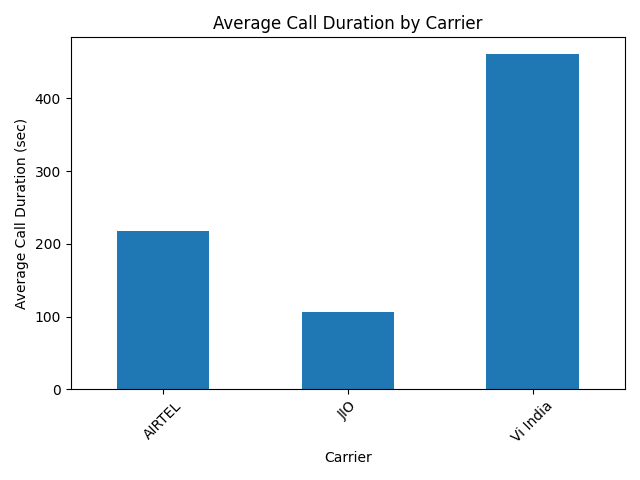
\includegraphics[width=0.5\linewidth]{avg_duration_by_carrier.png}
    \caption{Average call duration across carriers}
    \label{fig:cd}
\end{figure}

An important indicator of network reliability is the call drop rate. The comparison across carriers is shown in \autoref{fig:dr}. We observe that Jio exhibits a relatively higher drop rate compared to the other carriers. VI India reports a drop rate of zero; however, this result should be interpreted cautiously since only one VI user participated in the pilot study, making the sample size insufficient for a reliable conclusion.

\begin{figure}[h]
    \centering
    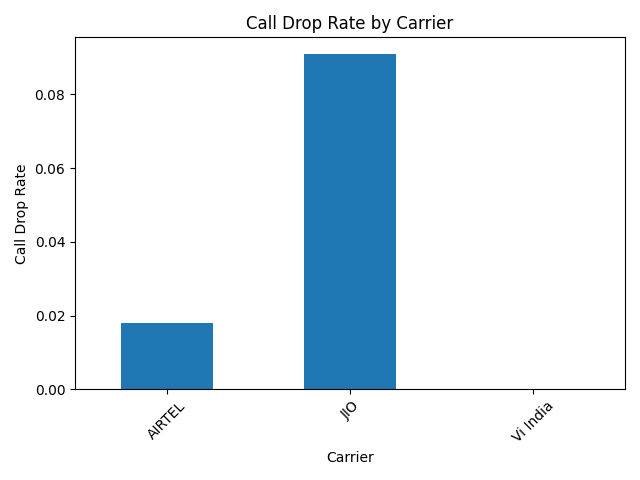
\includegraphics[width=0.5\linewidth]{drop_rate_by_carrier.png}
    \caption{Call drop rate across carriers}
    \label{fig:dr}
\end{figure}

We further analyze the distribution of audio-related issues reported by users for each carrier, as illustrated in \autoref{fig:ai}. The category ``UNKNOWN'' corresponds to calls where users did not explicitly report any audio issue. Across all carriers, the majority of calls fall under either the ``UNKNOWN'' or ``CALL PERFECT'' categories, indicating that most calls were perceived to have acceptable quality. Nevertheless, approximately 10--15\% of calls (depending on the carrier) were associated with noticeable audio issues.

\begin{figure*}[!t]
    \centering
    
    \subfigure[Audio issues reported for Airtel]{
        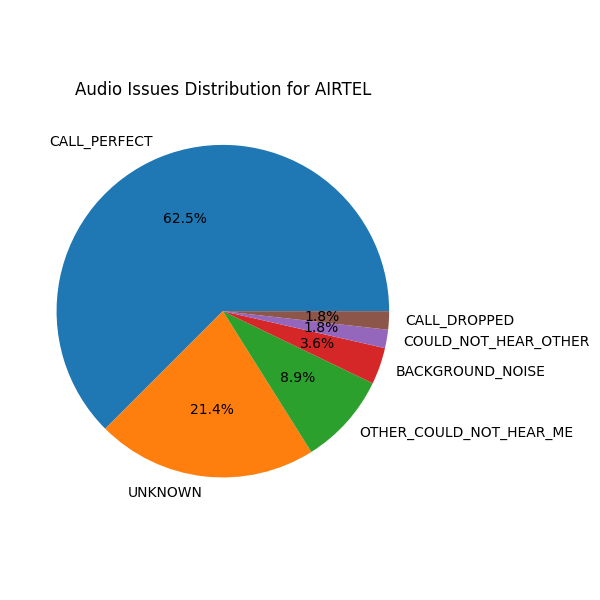
\includegraphics[width=0.30\linewidth]{audio_issues_distribution_AIRTEL.png}
        \label{fig:air}
    }
    \hfill
    \subfigure[Audio issues reported for Jio]{
        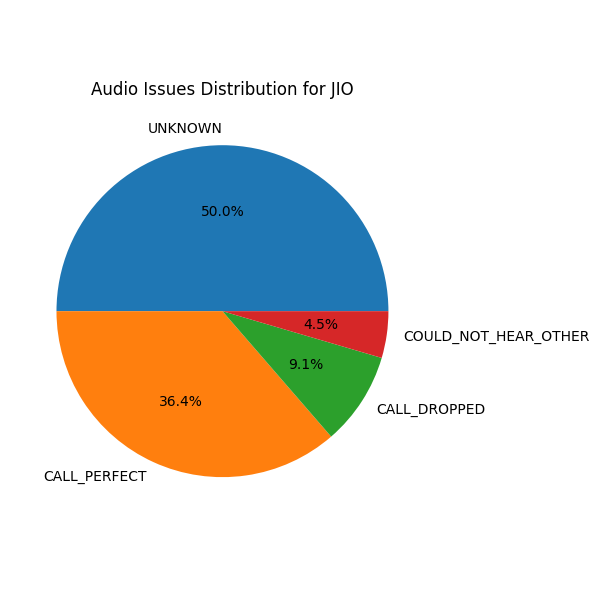
\includegraphics[width=0.30\linewidth]{audio_issues_distribution_JIO.png}
        \label{fig:jio}
    }
    \hfill
    \subfigure[Audio issues reported for VI India]{
        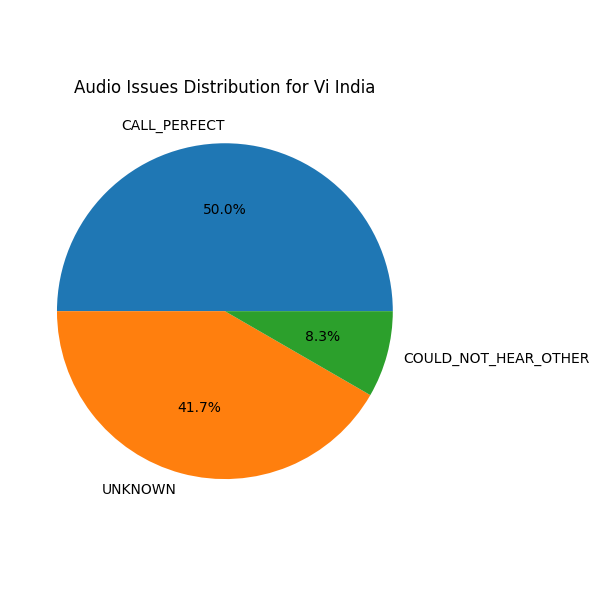
\includegraphics[width=0.30\linewidth]{audio_issues_distribution_Vi India.png}
        \label{fig:vi}
    }
    
    \caption{Distribution of reported audio issues across carriers}
    \label{fig:ai}
\end{figure*}

Finally, \autoref{fig:io} and \autoref{fig:ng} present additional characteristics of the collected data. The indoor/outdoor distribution provides insights into the environments in which calls were placed, while the network generation analysis highlights the proportion of calls conducted over WiFi and cellular networks. In particular, a significantly larger fraction of Airtel calls were placed using WiFi compared to Jio and VI India. This may partially explain the comparatively higher voice quality ratings observed for Airtel users.

\begin{figure*}[!t]
    \centering
    \subfigure[Indoor and outdoor calls by carrier]{
        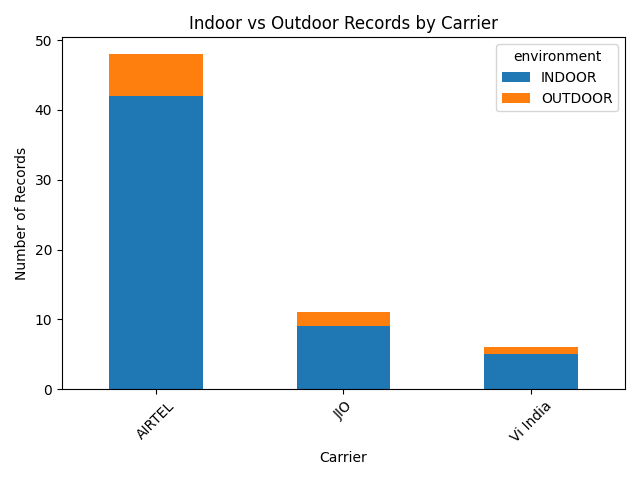
\includegraphics[width=0.45\linewidth]{indoor_outdoor_by_carrier.png}
        \label{fig:io}
    }
    \hfill
    \subfigure[Network generation used across carriers]{
        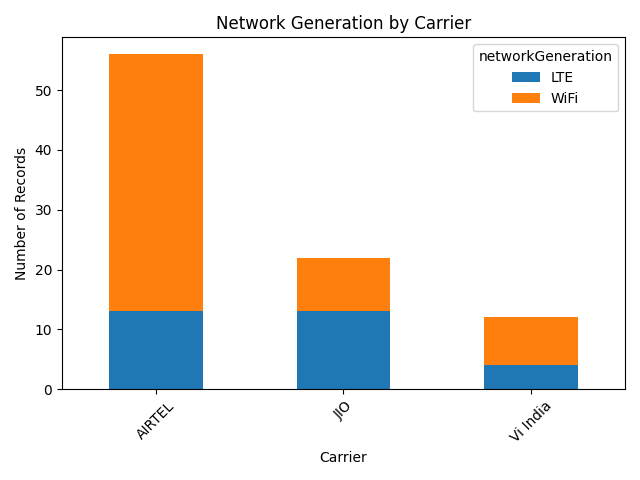
\includegraphics[width=0.45\linewidth]{network_generation_by_carrier.png}
        \label{fig:ng}
    }
    \caption{Additional characteristics of the collected dataset}
\end{figure*}
We couldn't reliably gather signal strength and location data since our sample size was small, and users mostly keep their location turned off.

\section{Conclusion}

In this work, we presented a pilot study for analyzing user-perceived voice call quality across different telecom carriers using data collected through our mobile application. The collected dataset enabled us to study multiple aspects of call performance, including perceived voice quality, call drop rates, audio-related issues, and the impact of different network generations.

Although the current study was conducted on a relatively small group of pilot users, the proposed system can be naturally scaled to a much larger user base. Collecting data from a broader and more diverse population would enable more reliable statistical analysis and provide deeper insights into regional network performance, carrier reliability, and user experience trends. Such large-scale deployment could help users make informed decisions regarding network providers and could also assist telecom operators in identifying and addressing quality-of-service issues more effectively.


\section{Acknowledgments}
We would like to thank Prof. Bhaskaran Raman for taking out his precious time and guiding us throughout our project.


\nocite{langley00}

\bibliography{example_paper}
\bibliographystyle{icml2025}


%%%%%%%%%%%%%%%%%%%%%%%%%%%%%%%%%%%%%%%%%%%%%%%%%%%%%%%%%%%%%%%%%%%%%%%%%%%%%%%
%%%%%%%%%%%%%%%%%%%%%%%%%%%%%%%%%%%%%%%%%%%%%%%%%%%%%%%%%%%%%%%%%%%%%%%%%%%%%%%
% APPENDIX
%%%%%%%%%%%%%%%%%%%%%%%%%%%%%%%%%%%%%%%%%%%%%%%%%%%%%%%%%%%%%%%%%%%%%%%%%%%%%%%
%%%%%%%%%%%%%%%%%%%%%%%%%%%%%%%%%%%%%%%%%%%%%%%%%%%%%%%%%%%%%%%%%%%%%%%%%%%%%%%

%%%%%%%%%%%%%%%%%%%%%%%%%%%%%%%%%%%%%%%%%%%%%%%%%%%%%%%%%%%%%%%%%%%%%%%%%%%%%%%
%%%%%%%%%%%%%%%%%%%%%%%%%%%%%%%%%%%%%%%%%%%%%%%%%%%%%%%%%%%%%%%%%%%%%%%%%%%%%%%


\end{document}






\documentclass{article}
\usepackage{graphicx} % Required for inserting images

\title{RnD Project Report \\ 
Call Feedback App}
\author{Gaurav Kumar \\ Shiv Narang}
\date{February 2026}

\begin{document}

\maketitle


\end{document}
